\documentclass[%
	%twocolumn,
	pdftex,%              PDFTex verwenden da wir ausschliesslich ein PDF erzeugen.
	a4paper,%             Wir verwenden A4 Papier.
	landscape,%						Seite - Landscape
	ngerman,
	oneside,%             Einseitiger Druck.
	4pt,%                 Grosse Schrift, besser geeignet f�r A4.
	halfparskip,%         Halbe Zeile Abstand zwischen Abs�tzen.
]{scrbook}



\usepackage[utf8]{inputenc}

\usepackage{amssymb}
\usepackage{amsfonts}
\usepackage{verbatim}
\newcommand{\changefont}[3]{
\fontfamily{#1} \fontseries{#2} \fontshape{#3} \selectfont}

\usepackage[none]{hyphenat}
\sloppy

\usepackage{graphicx}

\usepackage[ngerman]{babel}
%\usepackage{a4wide}
\usepackage{multicol}
%\usepackage{epsfig}
% um eps-einzubinden
\usepackage[landscape]{geometry}

\usepackage{array}

\usepackage[fleqn]{amsmath}
%\usepackage{marvosym}
%\uspackage{amsopn}

\usepackage{color}
\usepackage{tabularx}

\usepackage{fancyvrb} %\usepackage{fancybox}

\usepackage{lmodern}

\usepackage{framed}

\usepackage{listings}             % Include the listings-package

\definecolor{mygreen}{rgb}{0,0.6,0}
\definecolor{mymauve}{rgb}{0.58,0,0.82}
\definecolor{lightgrey}{gray}{0.6}
\definecolor{lightgray}{rgb}{.9,.9,.9}
\definecolor{darkgray}{rgb}{.4,.4,.4}
\definecolor{purple}{rgb}{0.65, 0.12, 0.82}

\lstdefinelanguage{JavaScript}{
	keywords={break, case, catch, continue, debugger, default, delete, do, else, false, finally, for, function, if, in, instanceof, new, null, return, switch, this, throw, true, try, typeof, var, let, void, while, with},
	morecomment=[l]{//},
	morecomment=[s]{/*}{*/},
	morestring=[b]',
	morestring=[b]",
	ndkeywords={class, export, boolean, throw, implements, import, this},
	keywordstyle=\color{blue}\bfseries,
	ndkeywordstyle=\color{purple}\bfseries,
	identifierstyle=\color{black},
	commentstyle=\color{mygreen}\ttfamily,
	stringstyle=\color{red}\ttfamily,
	sensitive=true
}

\lstset{ %
	backgroundcolor=\color{white},   % choose the background 
	basicstyle=\linespread{0.9}\scriptsize,
	language=JavaScript,
	keywordstyle=\color{blue},       % keyword style
	commentstyle=\color{mygreen},       % keyword style
	stringstyle=\color{mymauve},
	frame=single,
	framerule=1px,
	rulecolor=\color{spec_gray}, 
	aboveskip=\smallskipamount, 
	belowskip=\smallskipamount,       % 
	tabsize=1,	                   % sets default tabsize to 2 
}

%\usepackage[retainorgcmds]{IEEEtrantools} %IEEEeqnarray

\usepackage{xfrac} %f"ur sch"one 1/2 etc. Br"uche: \sfrac{1}{2}
\usepackage{cancel} %Durchstreichen in amsmath: \cance{x} oder \cancelto{0}{x}
\usepackage{enumitem}

\definecolor{spec_gray}{gray}{0.5}
\definecolor{spec_lgray}{gray}{0.65}
\definecolor{spec_blue}{rgb}{0,0.37,1}
\definecolor{spec_red}{rgb}{1,0.1,0.1}
\definecolor{spec_llgray}{gray}{0.9}

\newenvironment{bspbox}{%
  \def\FrameCommand{\fboxrule 1pt \colorbox{spec_llgray}}%
  \MakeFramed {\advance\hsize-\width \FrameRestore}}%
 {\endMakeFramed} 
 
% cp850 fr DOS, ansinew fr Windows statt latin1
%\renewcommand{\familydefault}{phv}
% setzt Helvetica (sieht aus wie Arial und sieht auch nach dvi2pdf noch gut aus)

\newcommand{\bsp}[1]{\vspace{-1.5mm}\begin{bspbox}\textbf{Bsp.:}  #1\end{bspbox}\vspace{-1mm}}

\newenvironment{mainbox}{%
  \def\FrameCommand{\fboxrule 1px \fcolorbox{black}{spec_blue}}%
  \MakeFramed {\advance\hsize-\width \FrameRestore}}%
 {\endMakeFramed}
 
\newenvironment{subbox}{%
  \def\FrameCommand{\fboxrule 1px \fcolorbox{black}{spec_gray}}%
  \MakeFramed {\advance\hsize-\width \FrameRestore}}%
 {\endMakeFramed}

\newenvironment{subsubbox}{%
  \def\FrameCommand{\fboxrule 1px \fcolorbox{black}{spec_lgray}}%
  \MakeFramed {\advance\hsize-\width \FrameRestore}}%
 {\endMakeFramed}
 
\newenvironment{titlebox}{%
  \def\FrameCommand{\fboxrule 1pt \fcolorbox{black}{black}}%
  \MakeFramed {\advance\hsize-\width \FrameRestore}}%
 {\endMakeFramed} 
 
% cp850 fr DOS, ansinew fr Windows statt latin1
%\renewcommand{\familydefault}{phv}
% setzt Helvetica (sieht aus wie Arial und sieht auch nach dvi2pdf noch gut aus)

\newcommand{\maintopic}[1]{\setcounter{subtopicenum}{0}\setcounter{subsubtopicenum}{0}\vspace{-4px}\begin{mainbox}\textcolor{white}{\textbf{\large{\stepcounter{maintopicenum}\Roman{maintopicenum}. #1}}}\end{mainbox}\vspace{-4px}}

\newcommand{\subtopic}[1]{\setcounter{subsubtopicenum}{0}\vspace{-4px}\begin{subbox}\textcolor{white}{\textbf{\stepcounter{subtopicenum}\Roman{maintopicenum}.\arabic{subtopicenum} #1}}\end{subbox}\vspace{-4px}}

\newcommand{\subsubtopic}[1]{\vspace{-3px}\begin{subsubbox}\textcolor{white}{\textbf{\stepcounter{subsubtopicenum}\Roman{maintopicenum}.\arabic{subtopicenum}.\arabic{subsubtopicenum} #1}}\end{subsubbox}\vspace{-3px}}

\newcommand{\titletopic}[1]{\vspace{0px}\begin{titlebox}\textcolor{red}{\textbf{#1}}\end{titlebox}\vspace{-3px}}

\newcommand{\vect}[1]{\mathbf{#1}}
\newcommand{\arcsinh}{\operatorname{arcsinh}}
\newcommand{\arccosh}{\operatorname{arccosh}}
\newcommand{\artanh}{\operatorname{artanh}}
\newcommand{\grad}{\operatorname{grad}}
\newcommand{\divergenz}{\operatorname{div}}
\newcommand{\rot}{\operatorname{rot}}
\newcommand{\D}{\,\textrm{d}}
\newcommand{\spec}{\operatorname{spec}}

\renewcommand\arraystretch{1.5}

\CustomVerbatimEnvironment{myverbatim}{Verbatim}{fontsize=\footnotesize,baselinestretch=0.8,numbers=none,showspaces=false,frame=single,rulecolor=\color{spec_gray}}     

\newenvironment{tight-itemize}
{ \begin{itemize}[leftmargin=*, nosep]
    \setlength{\itemsep}{0px}
    \setlength{\parskip}{0px}
    \setlength{\parsep}{0px}  }
{ \end{itemize}                  } 

\oddsidemargin-2.2cm
\evensidemargin-2.2cm
\textwidth29cm
\headheight0cm
\topmargin-2.8cm
\textheight20cm
\parskip0cm
\parindent0cm

\parskip-0.5mm

\pagestyle{empty}
%\pagenumbering{arabic}

\begin{document}\changefont{cmss}{m}{n}

\newcounter{maintopicenum}
\newcounter{subtopicenum}
\newcounter{subsubtopicenum}

\begin{multicols}{4}[][-5pt]

\setlength{\abovedisplayshortskip}{-0px}
\setlength{\abovedisplayskip}{-0px}
\setlength{\belowdisplayskip}{-0px} %Mathmode-Commands zum Platz sparen
\setlength{\arraycolsep}{2mm}

\setlength{\topsep}{4px} %Platz sparen bei Titeln
%\setlength{\parsep}{-20mm}

\raggedbottom %whitespace am Ende der letzten Seite statt verteilen des Inhalts auf ben"otigte Seiten


\titletopic{WED3 Zusammenfassung \qquad \today \\ HSR FS17}
%\qquad \LaTeX{} Design Martin Stypinski
\maintopic{Introduction of Web}
\subtopic{Benefits}
\begin{tight-itemize}
	\item{No need for backup} 
	\item{Platform independent} 
	\item{No software update} 
	\item{Lower investment costs} 
	\item{Software as a Service} 
\end{tight-itemize}
\subtopic{Liabilities}
\begin{tight-itemize}
	\item{No data sovereignity}
	\item{Limited calibration possibilities} 
	\item{Limited/restricted hardware access} 
	\item{No operation system access} 
	\item{More expensive deployment strategies} 
\end{tight-itemize}
\maintopic{What is Routing?}
\begin{tight-itemize}
	\item{Links multiple application parts together}
	\item{Provides the concept of information architecture (IA)}
\end{tight-itemize}
\subtopic{Basics}
\begin{tight-itemize}
	\item{Routing is accomplished \textbf{completely} client-side}
	\begin{tight-itemize}
		\item{No page reload, no roundtrip, server isn't involved}
		\item{Page transition is managed by JS completely}
		\item{Working back-button and bookmarks}
	\end{tight-itemize}
	\item{Entry Point [View UI controller] is enforced by the given route}
	\begin{tight-itemize}
		\item{Controller provides features behind a View (UI) and bootstraps it}
	\end{tight-itemize}
	\item{Router provides client-side event hooks during navigation} - Lifecycle management
\end{tight-itemize}
\subtopic{Client-side routing concepts}
\begin{tight-itemize}
	\item{\textbf{The old way}} - Earlier, we used anchors (\#). Don't use these anymore!
	\item{\textbf{The HTML5 way}}
	\begin{tight-itemize}
		\item{JavaScript API {\texttt window.history } is used}
		\item{{\texttt window.history.pushState} causes the address bar to show the URL, but won't cause the browser to load it (or even check, if it's valid)}
		\item{{\texttt window.onpopstate} can be used to listen for route changes}
		\item{\textbf{warning:} configuration adjustments needed on server-side (all sub-routes must return root-files)}
	\end{tight-itemize}
\end{tight-itemize}
\subtopic{Example routeConfig}
\lstinputlisting[label={routeConfig.js}, caption={routeConfig.js}, language={JavaScript}]{./sourcecode/routing/routeConfig.js}
\maintopic{Data Bindings}
\lstinputlisting[language={HTML}]{./sourcecode/bindings/example_binding.html}
\lstinputlisting[language={JavaScript}]{./sourcecode/bindings/example_binding.js}
\maintopic{Services}
\begin{tight-itemize}
	\item{\ldots contain the major application logic}
	\item{\ldots are generally the source of all application data \textbf{Data Services}}
	\item{Provide microtesting of smalles possible logic units}
	\item{Completely decoupled from UI}
	\item{\textbf{UI Services}} are usually seen in the communication between UI controllers.
\end{tight-itemize}
\lstinputlisting[language={JavaScript}]{./sourcecode/controllers/example_controller.js}
\maintopic{Bundling SPAs}
\begin{tight-itemize}
	\item{All JS code must be delivered to the client over potentially metered/slow networks}
	\item{Bundling and minifying the source leads to smaller SPA footprint}
	\item{Larger SPAs with many modules need a reliable dependency management}
	\item{Initial footprint can be reduced by loading dependent modules on-demand}
\end{tight-itemize}
\subtopic{WebPack as bundler}
\begin{tight-itemize}
	\item{\textbf{Entry}} - The entry point (modules to be bundled) tells webpack where to start and follows the graph of dependencies to know what to bundle.
	\item{\textbf{Output}} - Tell webpack where to bundle your application
	\item{\textbf{Loaders}} - Loaders in webpack transform these files into modules as they are added to your dependency graph.
	\item{\textbf{Plugins}} - Loaders only execute transformations on a per-file basis, plugins are most commonly used performing actions and custom functionality.
\end{tight-itemize}
\lstinputlisting[label={webpack.js}, caption={webpack.js}, language={JavaScript}]{./sourcecode/bundling/example_webpack.js}
\maintopic{Angular 2}
\subtopic{Angular CLI}
\begin{lstlisting}
npm install -g @angular/cli // Install the CLI globally
ng new my-app // Create a new angular app
ng serve --open // Serve the Angular app and open the browser
ng build // Just build the angular app
ng test // Build the angular app and execute the test runner
ng generate module core
\end{lstlisting}
\subtopic{Architectural Overview}
\begin{tight-itemize}
	\item{\textbf{Modules}} - A cohesive block of code dedicated to closely related set of capabilities.
	\item{\textbf{Directives}} - Provides instructions to transform the DOM.
	\item{\textbf{Components}} - A component is a directive-with-a-template; it controls a section of the view.
	\item{\textbf{Templates}} - A template is a form of HTML that tells Angular how to render the component.
	\item{\textbf{Metadata}} - Describes a class and tells Angular how to process it.
	\item{\textbf{Services}} - Provides logic of any value, function or feature that your application needs.
\end{tight-itemize}
\subtopic{About Modules}
\begin{tight-itemize}
	\item{Every app has at least one Angular module (the \textbf{root} Module)}
	\item{Modules export features (directives, services, ...) required by other modules}
	\item{NICHT zu verwechseln mit ES6 Modules (ES6=pro file; Angular=logischer Block von mehreren ES6 Modulen)}
	\item{Library Modules:}
	\begin{tight-itemize}
		\item{May accomodate multiple Angular modules}
		\item{Contain and export also other facilities (classes, functions, \ldots)}
		\item{Angular ships as multiple library modules (all with the @angular-prefix)}
		\item{As an ES6 module, the module library provides single export with all containing features (also known as \textbf{barrel} export)}
	\end{tight-itemize}
\end{tight-itemize}
\subtopic{Modules}
\begin{tight-itemize}
  \item{\textbf{Root Module}} - By convention named AppModule (app.module.ts). Provides the main view, called the root component, that hosts all other app views. Is bootstrapped by the main.ts
  \item{\textbf{Core Module}} - Provides globally required services and components directly needed by the root module. The core module should help keep the Root Module clean. Only the root Module should import the Core Module.
  \item{\textbf{Shared Module}} - Provides globally used components/directives/pipes. It's a global UI component module. Do not specify app-wide singleton providers (services) in a shared module (use Root Module instead).
  \item{\textbf{Feature Module}} - Splits the application into cohesive feature sets. Allows to assign development responsibilities to different teams. Feature modules are designed to extend the app. A feature module can expose or hide it's implementation from other modules.
  \item{\textbf{Lazy Module}} - Provides similar features such as Feature Modules. Reduces initial footprint of your SPA. Lazy loaded when invoked by a lazy route. Has it's own DI Container (a child of the root injector).
\end{tight-itemize}
\lstinputlisting[label={App Module Code}, caption={app.module.ts}, language={JavaScript}]{./sourcecode/testat/angular/app.module.ts}
\lstinputlisting[label={Dashboard Module Code}, caption={dashboard.module.ts}, language={JavaScript}]{./sourcecode/testat/angular/dashboard.module.ts}
\subtopic{@NgModule() Metadata}
\begin{tight-itemize}
	\item{\texttt{declarations[Type1, Type2, \ldots]}} - The \textit{view classes} that belong to this module. Angular has 3 view classes: components, directives and pipes.
	\item{\texttt{exports[Type1, Type2, Module1, Module2, \ldots]}} - The subset of declarations that should be visible and usable in the component templates of other modules. Can re-export other modules, which are automatically included when importing this module.
	\item{\texttt{imports[Module1, Module2, \ldots]}} - Specifies the modules which exports/providers should be imported into \textit{this} module.
	\item{\texttt{providers[Provider1, Provider2, \ldots]}} - Creators of services that this module contributes to the global collection of services (Dependency injection container); they become accessible in all parts of the app.
	\item{\texttt{bootstrap[Component]}} - The main application view, called the \textit{root component}. Only the \textit{root module} should set this property (enables usage of the root HTML tag: \texttt{<app-root>}).
\end{tight-itemize}
\subtopic{Module metadata and provider accumulation mechanisms}
\begin{tight-itemize}
	\item{Default import} - Imports all components, Pipes, Directives from the given ForeignModule. \textit{Declarations will be re-instantiated on the current module level.} Providers are registered into the current DI container, if registration not yet made.
	\item{\texttt{forChild(config?)} import} - Represents a static method on a module class (by convention). It is nearly the same as a default import, but allows you to configure services for the current Module level. It returns an object with a \texttt{providers} property and an \texttt{ngModule} property.
	\item{\texttt{forRoot() import}} - Represents a static method on a module (by convention, see \texttt{\textbf{forChild()}} import). This type of import is useful when you want to enforce that the same provider \textbf{won't} be loaded twice by lazy modules.
	\begin{tight-itemize}
		\item{\textbf{Only root modules} should import foreign Modules by calling \texttt{forRoot()}}
		\item{Declare your providers in \texttt{@NgModule} declaration OR in \texttt{forRoot()}, but \textbf{never} in both.}
		\item{The \texttt{providers} are added to the DI container on \textbf{root} level}
		\item{Also, the other ForeignModule are imported by the \texttt{NgModule} property.}
		\item{Providers from \texttt{ForeignModule.forRoot()} take precedence over the \texttt{providers} from the module definition.}
	\end{tight-itemize}
\end{tight-itemize}
\subtopic{Components}
Components control and support the view (Controller in MVC / ViewModel in MVVM). Declared as a TS class with an \texttt{@Component} function decorator.
The lifecycle is managed by Angular (Hydration, Update, Dehydration)
\lstinputlisting[label={New Payment Components}, caption={payment.component.ts}, language={JavaScript}]{./sourcecode/testat/angular/new-payment.component.ts}
\subtopic{Templates}
\begin{tight-itemize}
  \item{Almost all HTML syntax is valid template syntax (except \texttt{<script>} for security reasons). Some legal HTML doesn't make much sense in a template (\texttt{<head>, <body>})}
  \item{Angular extends the HTML vocabulary of your templates with:}
  \begin{tight-itemize}
    \item{Interpolation}
    \item{Template Expression/Statements}
    \item{Binding Syntax}
    \item{Directives}
    \item{Template Reference Variables}
    \item{Template Expressoin Operators (Advanced)}
  \end{tight-itemize}
  \item{Binding Syntax}
  \begin{tight-itemize}
    \item{Two Way Binding [()]}: \texttt{<input type="text" [(ngModel)]="counter.team" $>$}
    \item{One Way (View to Model / Event Binding) (\ldots)}: \texttt{<button (click)="counter.eventHandler" $>$}
    \item{One Way (Model to View / Property Binding) [\ldots] or \{\{ \ldots \}\}: \texttt{<input type="text" [(ngModel)]="counter.team"$>$}}
  \end{tight-itemize}
  \item{Binding to targets must be declared as Inputs or Outputs (like in the example above)} 
\end{tight-itemize}
\subtopic{Directives}
Similar to a component, but without a template. Declares as a Typescript class with an \texttt{@Directive()} function decorator. Two different kind of directives exist: Strucutral directives (Modifies the structure of your DOM) and Attribute directives (Alter the appearance or behavior of an existing element)
\begin{tight-itemize}
  \item{Attribute Directive}
  \begin{tight-itemize}
    \item{\textbf{NgStyle Directive}} \texttt{<div [style.font-size]="isSpecial ? 'x-large' : 'smaller')>}
    \item{\textbf{NgClass Directive}} \texttt{<div [class.special]="isSpecial>} 
  \end{tight-itemize}
\item{Structural Directives}
	\begin{tight-itemize}
		\item{Asterisk is "syntactic sugar" for something a bit more complicated}
		\item{Angular desugars in two stages: First it translated the \texttt{*directive="..."} into a template \textit{attribute}, \texttt{template="directive ..."}. Then it translates the attribute into a \texttt{<template>} Element.}
		\item{Example: \texttt{<div *ngIf="hasTitle"$>$} results in\\ \texttt{<template [ngIf]="hasTitle"$>$<div>}} 
	\end{tight-itemize}
\end{tight-itemize}

\textbf{Template reference variables}
\begin{tight-itemize}
	\item{References a DOM element within a template}
	\item{Can also be a reference to an Angular component or directive}
	\item{Reference variables can be used anywhere in the template}
	\item{A hash symbol (\#) declares a reference variable}
	\item{Example:} 
	\begin{lstlisting}
		<input placeholder="phone number" #phone>
		<!-- phone refers to the input element -->
		<button (click)="callPhone(phone.value)">Call</button>
	\end{lstlisting}
\end{tight-itemize}
\subtopic{Services}
\begin{tight-itemize}
	\item Provides any value, function, or feature that your application needs.
	\item Almost anything can be a service - it should do one thing and do it well.
	\item Typical services are logging service, data service, message bus, tax calculator, application configuration
	\item Strongly coupled to Dependency Injection (Angular uses DI to provide the services to the components who need them. Therefore services must be registered in teh DI Container)\\
\end{tight-itemize}
Use the \texttt{@Injectable} decorator for services.
\begin{lstlisting}
@Injectable()
export class CounterService { }
\end{lstlisting}
Then you need to register the service within the DI contianer
\begin{lstlisting}
@NgModule({
	imports: [...],
	declarations: [...],
	providers: [ CounterService ],
	exports: [...]
})
export class CounterModule { }
\end{lstlisting}
To use the Service in a component, you can declare it in the constructor and it will be injected by the DI Container.
\begin{lstlisting}
@Component(...)
export class CounterComponent {
	private counter : CounterModel;
	constructor(private counterService: CounterService) {
		this.counter = counterService.load();
	}
}
\end{lstlisting}
\subtopic{Component Lifecycle}
Green events are more important
\begin{center}
	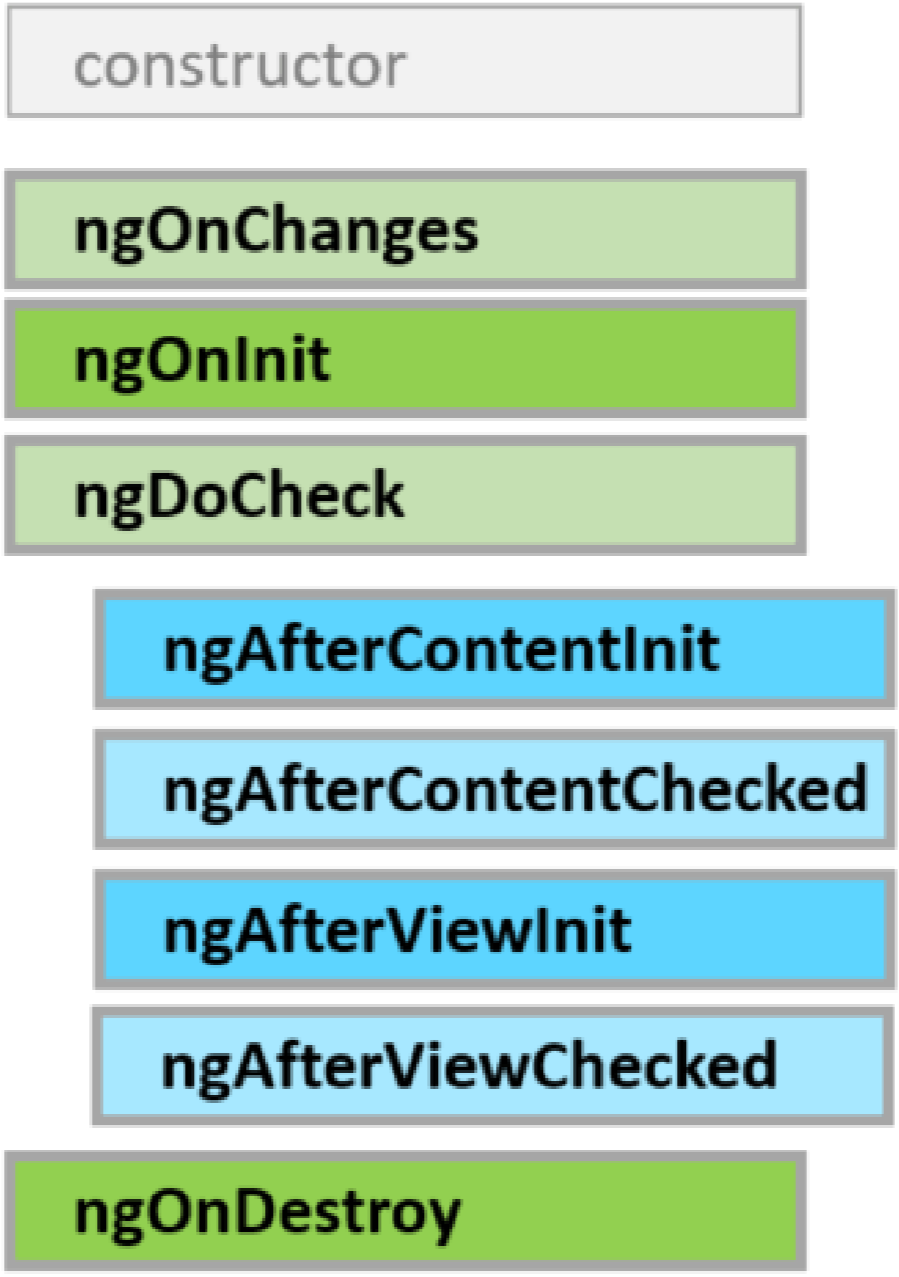
\includegraphics[width=0.1\textwidth]{img/ComponentLifecycle.png}
\end{center}
\begin{tight-itemize}
	\item \texttt{ngOnInit} - the creation event (also known as \textbf{hydration}) Setup the component and initially fetch data from an underlying data source (do not put too much logic here, just load data and delegate to other methods)
	\item \texttt{ngOnDestroy} - the destruction even (also known as \textbf{dehydration}) Use this method to detach event handlers to avoid memory leaks.
\end{tight-itemize}
\lstinputlisting[language={JavaScript}]{./sourcecode/angular/example_component.ts}
\subtopic{Component Transclusion}
Angular components consist of a view (HTML) and the component logic (Class). Reusable angular components enable parameterization of the view. Transclusion allows the component user to add content to the body section.
\begin{lstlisting}
<section>
	<wed-navigation>
		<h1 wed-title>WED3 Lecture</h1>
		<menu><!-- ... --></menu>
	</wed-navigation>
</section>
\end{lstlisting}
\begin{lstlisting}
<header>
	<ng-content select='[wed-title]'></ng-content>
</header>
<nav>
	<ng-content select='menu'><ng-content>
</nav>
\end{lstlisting}
\subtopic{Asynchronous Services}
In Angular, you can use RxJS or EventEmitters to handle async requests / responses. We'll focus on EventEmitters, where you have to subscribe to an event.
\begin{lstlisting}
@Injectables()
export class SampleService {
	public samplesChanged:EventEmitter<SampleModel[]> = 
		new EventEmitter<SampleModel[]>();
	load(): void {
		/* In real world, invoke data resource service here */
		this.sampleChanged.emit(this.samples);
	}
}
\end{lstlisting}
Receiving the data
\begin{lstlisting}
@Component({...})
export class SampleComponent implements OnInit, OnDestroy {
	ngOnInit() {
		this.samplesSubscription = this.samplesService
			.samplesChanged.subscribe(
				(data:SamplaModel[]) => { this.samples = data; } 
			}
	}
	ngOnDestroy() {
		this.sampleSubscription.unsubscribe();
	}
}
\end{lstlisting}
\subtopic{HTTP Client API with Observables}
\subparagraph{About Observables}
Think of an observable as a Stream: To listen to objects in the stream, subscribe to the observable. There are Hot Observables and Cold Observables. Hot Observables are shared among all subscribers (for sequences of events, such as mouse move or stock tickers). Cold Observables start running on subscription (such as async web requests) and are not shared among subscribers. They are automatically closed after the task is finished (as opposed to Hot Observables, which do not close automatically).
\subparagraph{Angular HTTP API} is implemented as a Cold Observable, therefore each subscription will result in a new HTTP Request. The \texttt{subscribe()} method listens for events of an Observable. This method consumes three function pointers:
\begin{tight-itemize}
	\item{onNext} - defines, what's to-do when data becomes available.
	\item{onError} - an error has been thrown while processing the observable. Depending on the implementation, the stream might be broken.
	\item{onComplete} - The task has been completed. The stream is about to be closed.
\end{tight-itemize}
\begin{lstlisting}
var subscription = this.http.get('api/samples').subscribe(
	function (x) { /* onNext -> data received (in x) */ },
	function (e) { /* onError -> the error (e) was thrown */ },
	function () { /* onCompleted-> the stream is closing down */ }
);
\end{lstlisting}
\lstinputlisting[language={JavaScript}]{sourcecode/angular/example_http.ts}
\subtopic{Angular Routing}
Use Angular Router to navigate among views. Once the application is bootstrapped, the Router performs the initial navigation based on the current browser URL. Angular Router is an external Module called RouterModule. It's important to add \texttt{<base href>} to the index.html site.
\subparagraph{Defining the Router Outlet}
RouterOutlet is a directive from the router library. It defines where the router should display the views. Can also be specified within a child component.
\lstinputlisting[language={HTML}]{sourcecode/angular/example_router_outlet.html}
\lstinputlisting[language={JavaScript}, label={Route Config}, caption={example-routing.module.ts}]{sourcecode/angular/example_routing.ts}
\subtopic{Angular Forms}
There are template driven and reactive (model-driven) forms. We focus on template driven forms.
By using the \texttt{<form>} tag, Angular automatically replaces it with an \texttt{ngForm}. It provides additional validation and error handling features. Use standard HTML5 features to validate your form. Use the \texttt{[(ngModel)]} binding to bind values. This reads out the value of the model for the first time. Updates are automatically written back into the bound model.
\lstinputlisting[language={HTML}]{sourcecode/angular/example_form.html}
\maintopic{React}
React ist eine Library (kein Framework!) um UI's zu bauen. Es besitzt ein minimales Featureset und wurde vom Gesichterbuch entwickelt.
\subparagraph{Prinzipien von React}
Functionale Programmierung: Komponenten sind Funktionen von \texttt{(Attribute, State?) => View}. Komposition statt Vererbung. Immutability. Minimieren von und expliziter mutable State. Braucht es einen State/Lifecycle? Dann verwende eine Klassenkomponente. Sonst verwende lediglich eine Funktion (\texttt{function Hello(props)}).
\subtopic{JavaScript XML (JSX)}
React verwendet JSX, einen Präprozessor, der JavaScript um XML ergänzt -- XML kann an beliebiger Stelle vorkommen.
\subparagraph{JSX Einschränkungen}
\begin{tight-itemize}
	\item{React Elemente müssen mit Grossbuchstaben anfangen. JavaScript-Keywords dürfen nicht verwendet werden.}
	\item{React muss immer importiert werden, wenn JSX verwendet wird. Weil JSX vom Präprozessor zu \texttt{React.createElement} Aufrufen umgewandelt wird.}
\end{tight-itemize}
\subtopic{Props and State}
Komponenten erhalten alle Parameter als \texttt{props} Objekt (bei Klasse als \texttt{this.props} und bei Funktionen als Parameter). \textbf{Props sind immer read-only}. React \textbf{Klassenkomponenten} können einen veränderbaren Zustand haben. Um den State zu ändern, verwenden wir die Methode \texttt{setState()}. Ist der nächste State vom Vorherigen abhängig, sollte man diese folgende Form verwenden (falls der neue State unabhängig vom alten ist, kann \texttt{state =$>$} weggelassen werden).
\lstinputlisting{sourcecode/react/example_counter.js}
\subtopic{React CLI}
\begin{lstlisting}
npm install -g create-react-app
create-react-app hello-hsr
npm start (Starts the development server)
npm run build (Bundles the app into static files for production)
npm test (Starts the test runner)
npm run eject (Removes this tool and copies build dependencies,
 config files, scripts into the app directory. If you do this, you can't go back!)
\end{lstlisting}
\subtopic{React Lifecycle}
\begin{tight-itemize}
	\item Mounting
	\begin{enumerate}
		\item \texttt{constructor(props)} - State initialisieren
		\item \texttt{render()}
		\item \texttt{componentDidMount()} - DOM aufgebaut, Remote Daten laden, setState führt zu Re-Rendering
	\end{enumerate}
	\item Updating
	\begin{enumerate}
		\item \texttt{componentWillReceiveProps(nextProps)} - Vorschau auf die nächsten Props.
		\item \texttt{shouldComponentUpdate(nextProps, nextState)} - wenn \texttt{return false}, wird Rendering übersprungen.
		\item \texttt{componentWillUpdate(nextProps, nextState)} - selten gebraucht (evtl. Animationen starten)
		\item \texttt{componentDidUpdate(prevProps, prevState)} - DOM ist aktualisiert.
	\end{enumerate}
	\item Unmounting
	\begin{enumerate}
		\item \texttt{componentWillUnmount()} - Aufräumen
	\end{enumerate}
\end{tight-itemize}

% Add white spaces inside the verbatim tag if you need to waste space (to keep the layout tidy).
\begin{verbatim}
\end{verbatim}
\end{multicols}

\end{document}
